\documentclass[11pt, aspectratio = 169]{beamer}

\usetheme[progressbar=frametitle]{metropolis}
\usepackage{appendixnumberbeamer}
\usepackage{booktabs}
\usepackage[scale=2]{ccicons}
\usepackage{pgfplots}
\usepgfplotslibrary{dateplot}
\usepackage{xspace}
\usepackage{hyperref}  
\usepackage{cancel}
\usepackage{tikz}  
\usetikzlibrary{shapes,decorations,arrows,calc,arrows.meta,fit,positioning}
\tikzset{
    -Latex,auto,node distance =1 cm and 1 cm,semithick,
    state/.style ={ellipse, draw, minimum width = 0.7 cm},
    point/.style = {circle, draw, inner sep=0.04cm,fill,node contents={}},
    bidirected/.style={Latex-Latex,dashed},
    el/.style = {inner sep=2pt, align=left, sloped}
}
\usepackage{verbatim} 
\usepackage{listings}
\newcommand{\themename}{\textbf{\textsc{metropolis}}\xspace}
\definecolor{links}{HTML}{1B1B81}
\hypersetup{colorlinks,linkcolor=blue,urlcolor=blue}

% listings: To highlight code:
\usepackage{listings}
\lstset{
  language=R,
  basicstyle=\ttfamily\footnotesize,
  keywordstyle=\color{blue},
  commentstyle=\color{green!50!black},
  stringstyle=\color{red},
  frame=single,
  showstringspaces=false
}
\lstset{basicstyle=\ttfamily\footnotesize, frame=single}

\title{Applied Economics}
\subtitle{Difference-in-Differences Estimator}
\author{Pello Aspuru}
\date{}
\institute{Winter 2025/26}
% \titlegraphic{\hfill\includegraphics[height=1.5cm]{logo.pdf}}
\setbeamercolor{normal text}{fg=black}
\setbeamercolor{block title}{fg=teal}
\setbeamercovered{transparent} % default faintness (~15%)

\let\svdescription\description
\let\svenddescription\enddescription
\renewenvironment{description}{%
  \svdescription%
  \let\svitem\item%
  \renewcommand\item[1][]{\svitem[\textcolor{\descriptioncolor}{##1}]}%
  }{
  \svenddescription%
  }
\newcommand\descriptioncolor{teal}

\begin{document}

\maketitle

\section{Introduction}

\begin{frame}{Introduction}
    
Four \color{teal}\textbf{quasi-experimental methods} \color{black}to \textit{mimic random treatment assignment:} 
\begin{enumerate}
    \item Instrumental variables (IV)
    \item Panel Data Methods
    \item Differences-in-differences (DiD)
    \item Regression discontinuity designs (RDD)
\end{enumerate}
\pause
\color{teal}\textbf{Panel Data Methods} \color{black} to control for unobserved time-invariant endogeneity $c_i$.
\begin{align*}
       Y_{it} = \beta_0 + \beta_1 X_{1,it} + c_i + \alert{\epsilon_{it}}, \quad i = 1, ... , n \quad t = 1, ... , T. 
\end{align*}
\vspace{-0.7cm}
\begin{itemize}
    \item[$\rightarrow$] What about time-varying endogenetiy $\alert{\epsilon_{it}}$?
\end{itemize} \pause
Today: \color{teal}\textbf{Differences in Differences} \color{black} methods.
\end{frame}

\begin{frame}{Differences-in-Differences}
Differences in Differences estimation requires a specific type of\alert{ panel data}:
\pause 
\begin{itemize}
    \item Time variation: all units are observed in two time periods. \pause
    \item Treatment variation: 
        \begin{itemize}
            \item Period 1: no unit receives treatment
            \item Period 2: some units are treated, others remain untreated (control group).
        \end{itemize}
\end{itemize}

Under certain assumptions, the control group can serve as the \textcolor{teal}{counterfactual} for the treatment group. $\rightarrow$ \textbf{Difference in outcomes between groups after vs. before treatment} gives causal effect of interest.
\end{frame}

\section{Example:  Causal effect of Minimum Wage on Employment}

\begin{frame}[fragile]{Card \& Krueger (1994)}
\begin{center}
        Does an increase in the minimum wage \alert{cause} a reduction in employment?
    \end{center}
\pause
\hyperlink{https://davidcard.berkeley.edu/papers/njmin-aer.pdf}{Card and Krueger (1994)} estimates the \alert{causal} effect of a minimum wage (MW) increase on the employment rate in the fast-food industry. 
\pause
\begin{itemize}
    \item New Jersey (NJ) increased the state MW in 1992 from \$4.25 to \$5.05 per hour \alert{(treatment group)}
    \item Neighboring Pennsylvania (PA) did not change its minimum wage level \\
    \alert{(control group)}
    \item The authors surveyed 410 fast-food establishments in NJ and eastern PA:
    \begin{itemize}
        \item First survey \alert{before} the NJ MW increase (February 1992), 
        \item Second survey \alert{after} the NJ MW increase (November 1992)
    \end{itemize} 
\end{itemize}
\pause
\vspace{0.3cm}
\begin{lstlisting}[language=R]
        df <- read.csv("./AE_week10_DD/df_min_wage.csv")
    \end{lstlisting}
\end{frame}

\begin{frame}[fragile]{Motivating Example}
    \begin{center}
        Does an increase in the minimum wage \alert{cause} a reduction in employment?
    \end{center}
    A Panel Data model to control for time-invariant endogeneity:
    \begin{align*}
       Y_{it} = \beta_0 + \beta_1 X_{1,it} + c_i + \alert{\epsilon_{it}}, \quad \quad i = 1, ... , n \quad \quad t = 1, 2. 
    \end{align*}
    \vspace{-0.6cm}
    \begin{itemize}
        \item [$Y_{it}$] Employment level in restaurant $i$ at time $t$
        \item [$X_{it}$] Indicator variable if restaurant $i$ experienced minimum wage increase at time $t$  \pause
        \item [$c_i$] Unobserved time-invariant characteristics of restaurant $i$ 
        \item [$\alert{\epsilon_{it}}$] Unobserved time-varying endogeneity.
    \end{itemize}
    \vspace{0.3cm}
    \begin{lstlisting}[language=R]
        panel_0 <- feols(emptot ~ is_min_wage_up | sheet, data = df)
    \end{lstlisting}
    \begin{itemize}
        \item[$\rightarrow$] Is exogeneity assumption $E[\alert{\epsilon_{it}}|X_{it}, c_i] = 0$ reasonable? Why?
    \end{itemize}
\end{frame}

\begin{frame}{Parallel Trends Assumption}

\begin{itemize}
    \item Panel methods control for time-invariant endogeneity $c_i$, but...
    \item We need to control for time-variying endogeneity $\alert{\epsilon_{it}}$.
\end{itemize}
\pause
\begin{center}
    How would employment have evolved \alert{over time} in NJ, \textit{had the minimum wage \textit{not} been increased}?
\end{center}
\pause
\begin{block}{Paralell Trends Assumption}
    \begin{itemize}
    \item[$\rightarrow$] Absent treatment, treated units would have followed the same trend as controls. \pause
    \item In our example: absent minimum wage increase, fast-food employment in NJ would have followed the same trend as in PA. \pause
    \item Is this assumption reasonable? 
    \begin{itemize}
        \item PA and NJ are very similar: similar institutions, similar habits, similar consumers, similar incomes, similar weather, etc.
    \end{itemize}
    \item Can we test this assumption with our dataset?
\end{itemize}
\end{block}
\end{frame}

\section{Visualizing Differences in Differences}

\begin{frame}[fragile]{DiD Estimator: Basic Form}

Start by grouping data into four groups:
\begin{lstlisting}[language=R]
    df_plot <- df %>%
                group_by(state, observation) %>%
                summarise(mean_emptot = mean(emptot, na.rm = TRUE),
                    sd_emptot = sd(emptot, na.rm = TRUE),
                    .groups = "drop")
\end{lstlisting}
\pause
    \centering
    \begin{table}
        %\caption{Sample Means of Employment (FTE) per Store}
        \begin{tabular}{lccc}
    \toprule
                           &  NJ & \only<3->{PA} & \\
                           \midrule
         Before Treatment  &  20.4 & \only<3->{23.3} & \\
After Treatment &  21.0 & \only<3->{21.2}  &\\
\midrule
Difference (A-B)& \only<2->{0.6} & \only<3->{-2.1} & \alert{\only<4->{DiD estimate: $0.6 - (-2.1) = 2.7$} }\\
\bottomrule
\end{tabular}
    \end{table}

\end{frame}

\begin{frame}[fragile]{Ussing \texttt{ggplot2} to Visualize DiD}

\begin{lstlisting}[language=R]
    ggplot(df_plot, aes(x = observation, y = mean_emptot, 
                        group = state, color = state)) +
    geom_line(linewidth = 0.5) +
    geom_point(size = 2) +
    scale_y_continuous(limits = c(16, 24)) +
    theme_minimal()
\end{lstlisting}

\end{frame}

\begin{frame}{DiD Estimator: Graphical}
\only<1>{   
    \begin{figure}
        \centering
        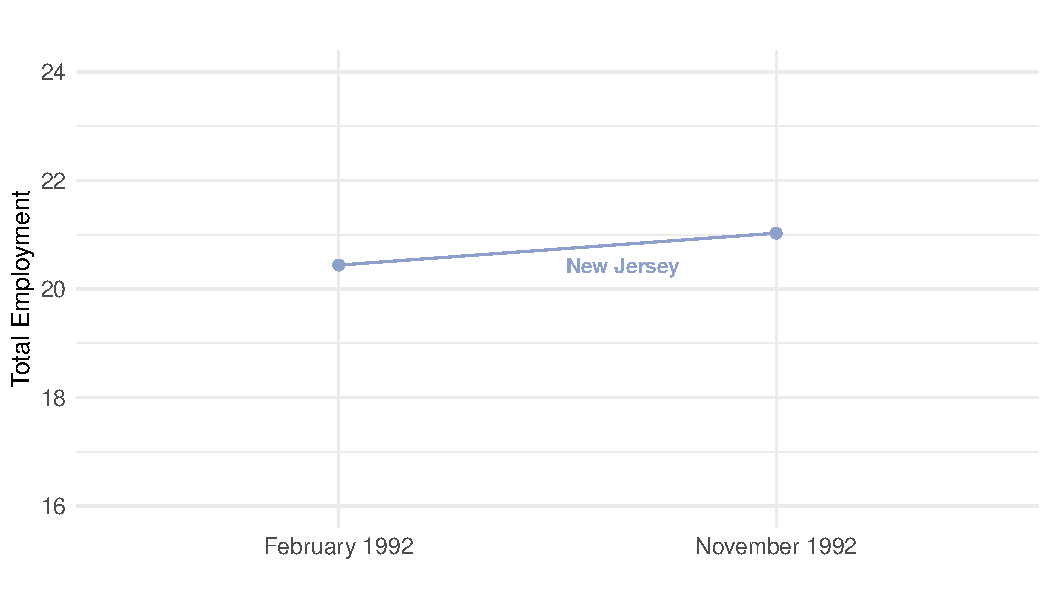
\includegraphics[width=0.9\linewidth]{DD_graph_1.pdf} 
    \end{figure}}
\only<2>{   
    \begin{figure}
        \centering
        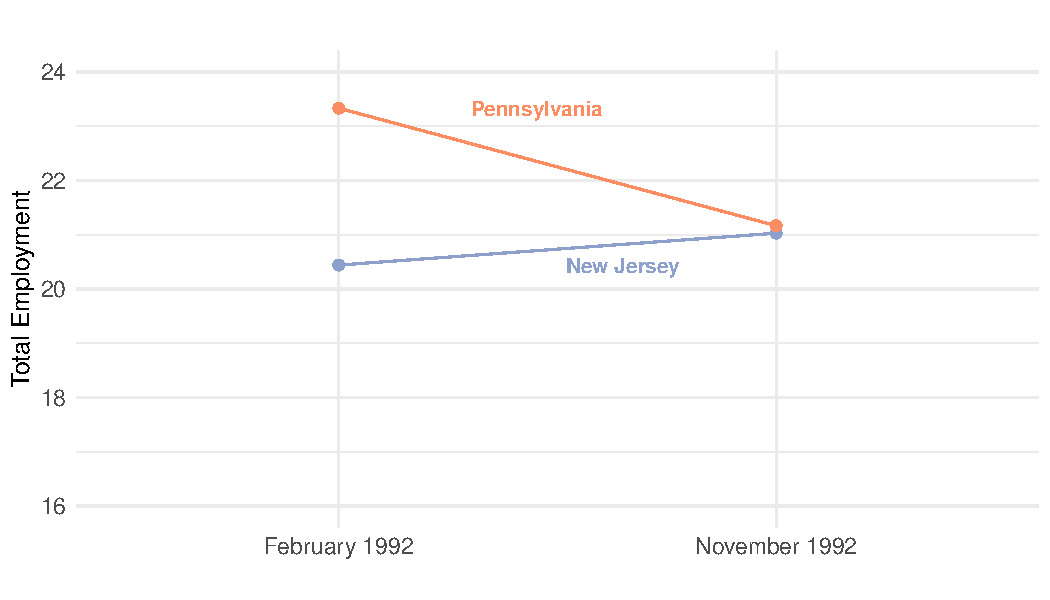
\includegraphics[width=0.9\linewidth]{DD_graph_2.pdf} 
    \end{figure}}
\end{frame}

\begin{frame}[fragile]{Adding the Paralell Trends Assumption}
    Obtain the time trend (i.e. slope) of Pennsylvania as \texttt{pa\_slope}
    \begin{lstlisting}[language=R]
pa_data <- df_plot %>% filter(state == "Pennsylvania")
pa_slope <- diff(pa_data$mean_emptot)
    \end{lstlisting} \pause
    Create a new \texttt{NJ\_counterfactual} dataset:
    \begin{lstlisting}[language=R]
NJ_counterfactual <- data.frame(
    observation = c("February 1992", "November 1992"),
    mean_emptot = c(nj_feb$mean_emptot, nj_feb$mean_emptot + pa_slope),
    state = "Counterfactual")
    \end{lstlisting} \pause
    Plot the counterfactual trend as an \textbf{additional line} of the previous code:
    \begin{lstlisting}[language=R]
geom_line(data = NJ_counterfactual, 
          aes(x = observation, y = mean_emptot, group = state),
          linetype = "dashed", linewidth = 0.5, color = "gray40") + ...
    \end{lstlisting}
\end{frame}

\begin{frame}{DiD Estimator: Graphical}
\only<1>{   
    \begin{figure}
        \centering
        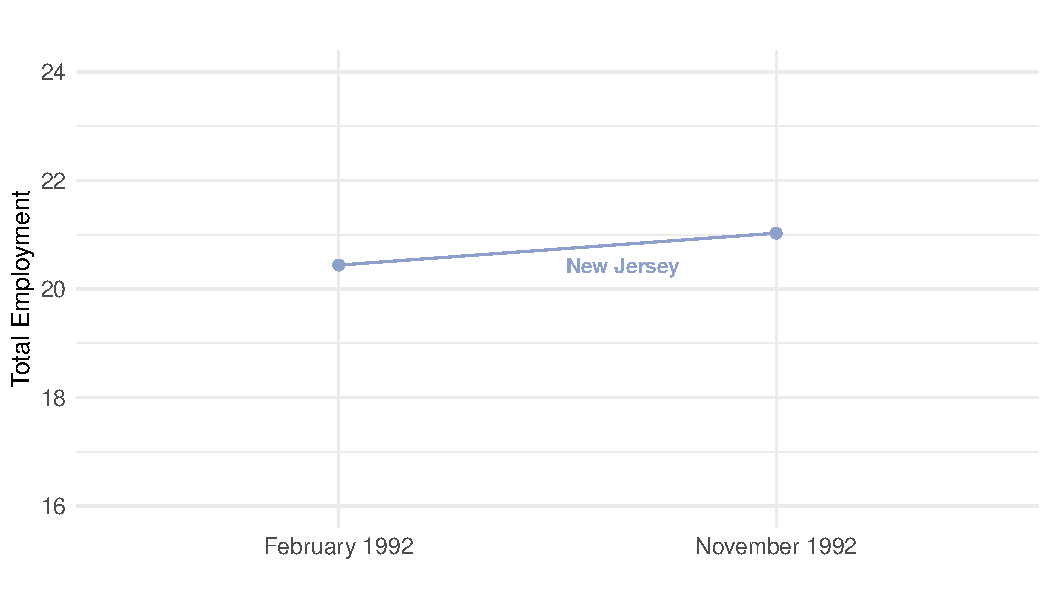
\includegraphics[width=0.9\linewidth]{DD_graph_1.pdf} 
    \end{figure}}
\only<2>{   
    \begin{figure}
        \centering
        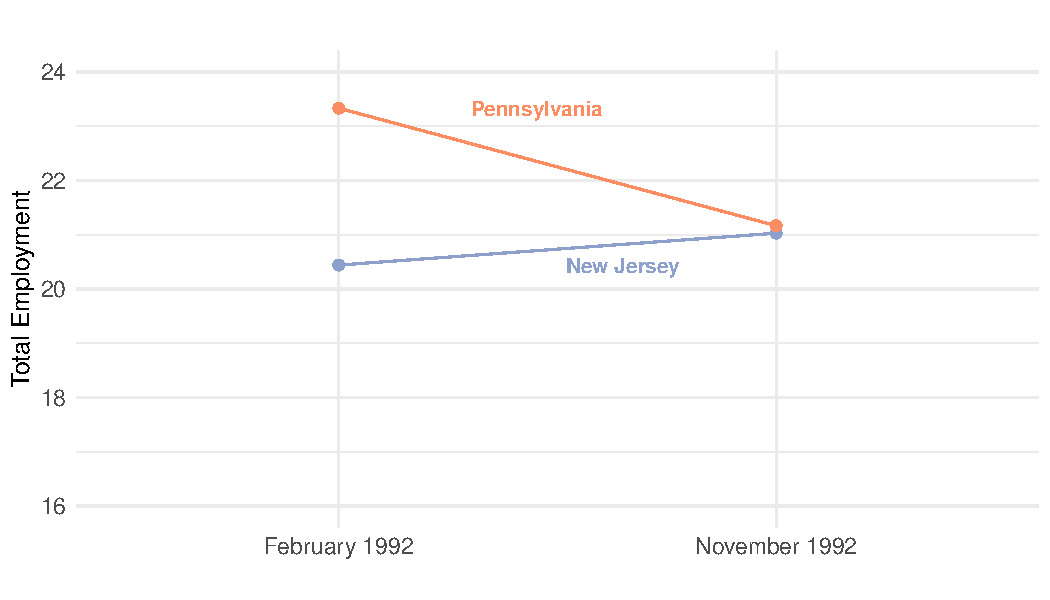
\includegraphics[width=0.9\linewidth]{DD_graph_2.pdf} 
    \end{figure}}
\only<3>{   
    \begin{figure}
        \centering
        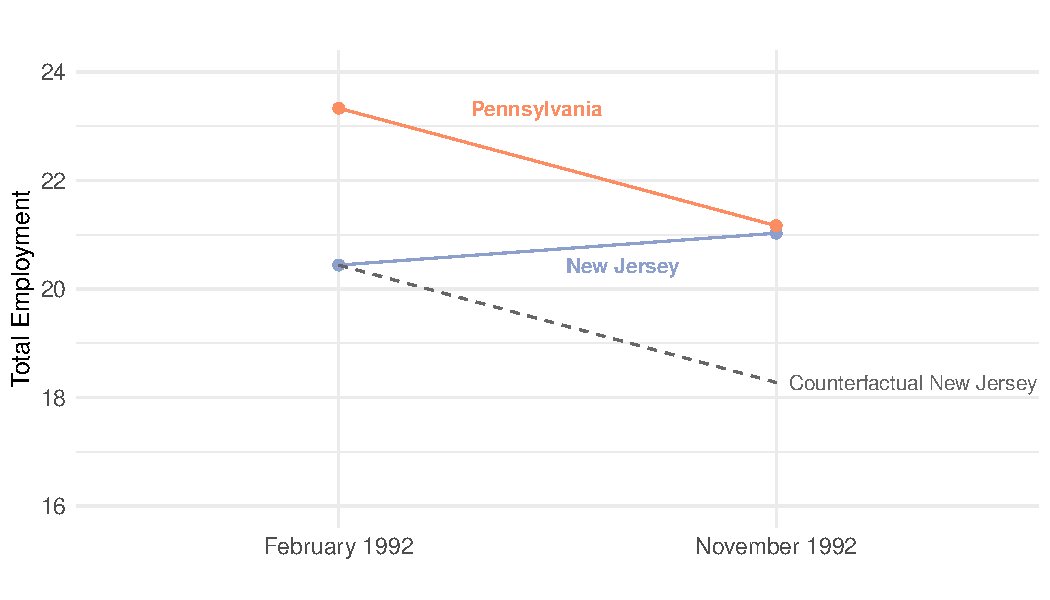
\includegraphics[width=0.9\linewidth]{DD_graph_3.pdf} 
    \end{figure}}
\end{frame}


\section{Diff-in-Diff Estimator: Basic Form}

\begin{frame}{DiD Estimator: Basic Form}
More generally, the DiD estimator is given as:
\begin{align*}
  \widehat{\beta}^{\text{DiD}} =& \, (\overline{Y}^{\text{treatment,after}} - \overline{Y}^{\text{treatment,before}}) - (\overline{Y}^{\text{control,after}} - \overline{Y}^{\text{control,before}}) \\
  =& \Delta \overline{Y}^{\text{treatment}} - \Delta \overline{Y}^{\text{control}} 
\end{align*}

with
\begin{description}
\item[$\overline{Y}^{\text{treatment,before}}$] sample average in the TG before the treatment \color{gray} $\rightarrow$ $\overline{Employm}^{\text{NJ,before}}$
\item[$\overline{Y}^{\text{treatment,after}}$] \color{black} sample average in the TG after the treatment \color{gray}
$\: \: \: \: \rightarrow$ $\overline{Employm}^{\text{NJ,after}}$
\item[$\overline{Y}^{\text{control,before}}$] \color{black} sample average in the CG before the treatment \color{gray} $\: \: \: \:  \rightarrow$ $\overline{Employm}^{\text{PA,before}}$
\item[$\overline{Y}^{\text{control,after}}$] \color{black} sample average in the CG after the treatment \color{gray} $\: \: \: \: \: \: \: \: \rightarrow$ $ \overline{Employm}^{\text{PA,after}}$
\end{description}
\end{frame}


\begin{frame}{Parallel Trends Assumption}
The crucial assumption to identify the causal effect of interest with the DiD estimator is the \alert{\textbf{Common or Parallel Trends Assumption:}}
\\
\textit{In the absence of treatment, time trends in the treatment group would have been the same as in the control group.}

\pause

Example: absent any minimum wage increase, Pennsylvania's fast-food employment trend would have been what we should have expected to see in New Jersey. $\rightarrow$ trend in PA is a reliable counterfactual for NJ

\pause

It is impossible to validate whether the assumption holds. (By definition, we cannot observe what would have happened in the absence of treatment in the TG) \\
Intuitive check: compare trends $before$ policy change

\end{frame}

\begin{frame}{Visualizing the Parallel Trends Assumption}
\only<1>{   
    \begin{figure}
        \centering
        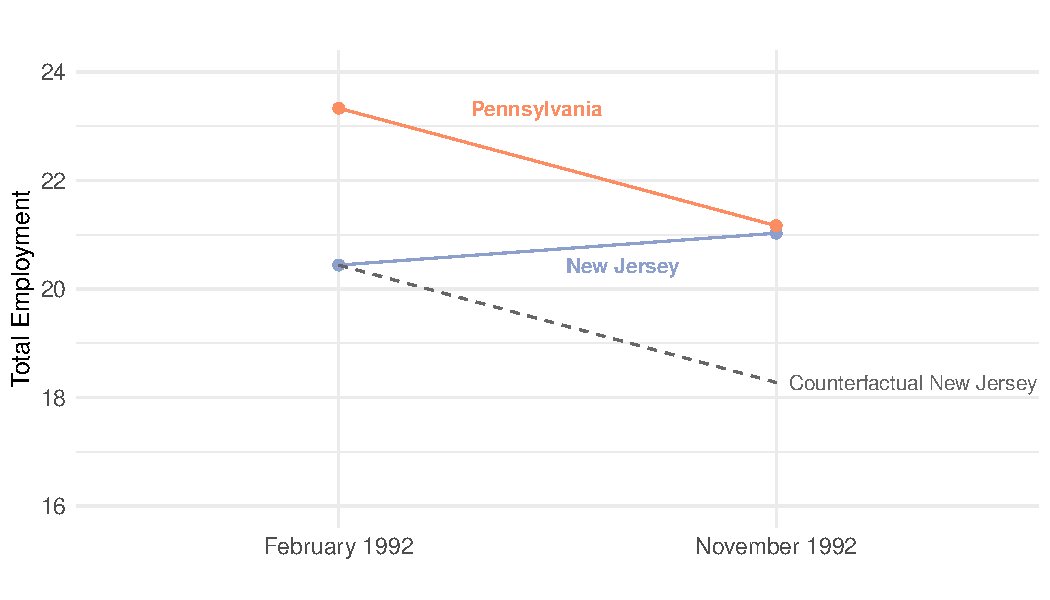
\includegraphics[width=0.9\linewidth]{DD_graph_3.pdf} 
    \end{figure}}
\only<2>{   
    \begin{figure}
        \centering
        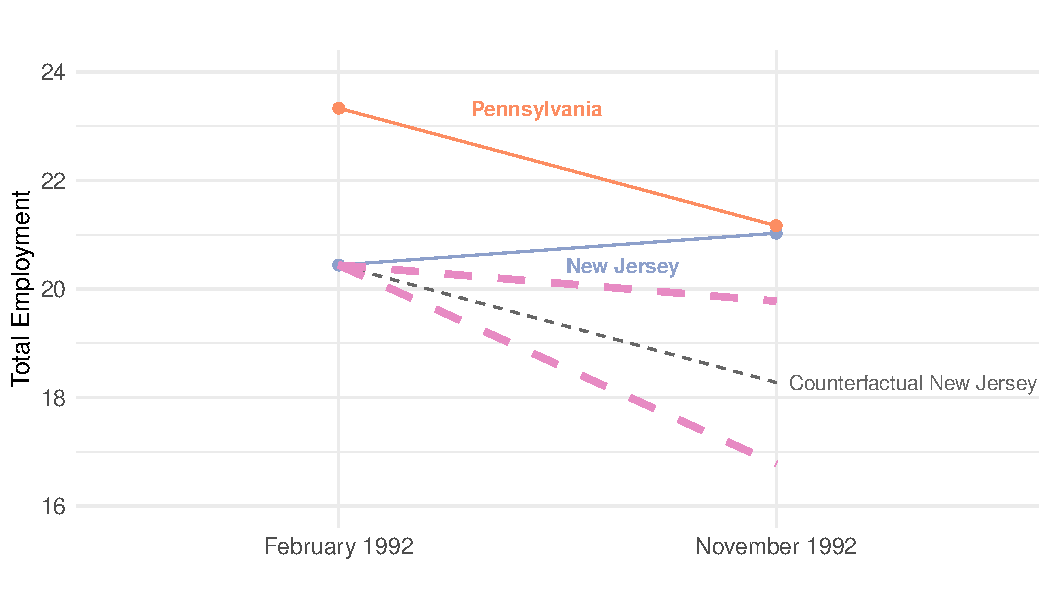
\includegraphics[width=0.9\linewidth]{DD_graph_4.pdf} 
    \end{figure}}
\end{frame}

\section{Diff-in-Diff Estimator: \\
Regression Form}

\begin{frame}[fragile]{Diff-in-Dif Estimator: Regression Form}
The simplets version of the DiD regression model is:
\vspace{-0.02cm}
\begin{align*}
  Y_{it}= & \alpha + \gamma Treat_i + \delta Post_t + \beta_{TE} (Post_t \times Treat_i) + \varepsilon_i 
\end{align*}
\begin{lstlisting}[language=R]
    did_model <- lm(emptot ~ time + treated + time:treated, data = df)
\end{lstlisting}
\vspace{-0.2cm}
\pause
\begin{description}
    \item[$Treat_i$] Treatment group dummy, with index $i$ for cross-sectional units
    $Treat_i = \begin{cases}
    0 & \text{if } i \text{ in Pennsylvania}, \\
    1 & \text{if } i \text{ in New Jersey}
    \end{cases}$
\item[$Post_t$] Treatment periods dummy, with index $t$ for time periods
    $Post_t = \begin{cases}
    0 & \text{if } t < \text{ April 1992,} \\
    1 & \text{if } t \geq \text{ April 1992}
    \end{cases}$
\item[$Treat_i \times Post_t$] Interaction term $\rightarrow$ the coefficient $\beta_{TE}$ is the DiD causal effect!
\end{description}
\end{frame}

\begin{frame}{Understanding the Regression}
\vspace{-0.2cm}
\begin{align*}
  Y_{it}=& \alpha + \gamma Treat_i + \delta Post_t + \beta_{TE} (Post_t \times Treat_i) + \varepsilon_i 
\end{align*}

Expeted outcomes in control units:
\begin{itemize}
    \item $E(Y_{it}|Treat_i=0,Post_t=0)= \alpha$
    \item $E(Y_{it}|Treat_i=0,Post_t=1)= \alpha + \alert{\delta}$
\end{itemize} \pause
Expected outcomes in treated units:
\begin{itemize}
    \item $E(Y_{it}|Treat_i=1,Post_t=0)= \alpha + \gamma$
    \item $E(Y_{it}|Treat_i=1,Post_t=1)= \alpha + \gamma  + \delta  + \beta_{TE}$
\end{itemize} 
\pause
The causal effect of the treatment on the treated, without the time trended is $\beta_{TE}$
\begin{align*}
    \underbrace{(\alpha + \gamma  + \delta  + \beta_{TE}) - (\alpha + \gamma)}_{\text{Effect of treatment on treated}}
    - 
    \underbrace{(\alpha -\alpha + \alert{\delta})}_{\text{Time trend}}
    = 
    \beta_{TE}
\end{align*}
\end{frame}



\begin{frame}[fragile]{Diff-in-Diff Estimator: Additional Controls}

\begin{itemize}
    \item Add controls $\alert{X_i}$ that measure pre-treatment characteristics of the units:
    \begin{align*}
    Y_{it}=& \alpha \;+\; \gamma Treat_i \;+\; \delta Post_t \;+\; \beta_{TE} (Post_t \times Treat_i) \;+\; \pi \alert{X_i} \;+\; \varepsilon_i 
    \end{align*}
    The additional regressors may lead to a more precise estimate of $\beta_{TE}$.
    \pause
    \vspace{1cm}
    \item Add unit-level fixed effects $\alert{FE_i}$ to control for all time-invariant unobservables:
    \begin{align*}
    Y_{it}=& \alpha \;+\; \gamma Treat_i \;+\; \delta Post_t \;+\; \beta_{TE} (Post_t \times Treat_i) \;+\; \alert{\sum_i \pi_i \alert{FE_i}} \;+\; \varepsilon_i 
    \end{align*} \pause
    \begin{lstlisting}[language=R]
    panel_1 <- feols(emptot ~ time + treated + is_min_wage_up | 
                    sheet, data = df)
    summary(panel_1, vcov = "hetero")
    \end{lstlisting}
\end{itemize}
\end{frame}

\begin{frame}{Summary}
\begin{itemize}
    \item DiD is a widely used quasi-experimental method to estimate causal effects when treatment is not randomly assigned.
    \item It requires \alert{panel data} on a treatment and a control group, as well as data for at least two time periods (before and after treatment).
    \item The key identifying assumption is the \alert{Parallel Trends Assumption}: in the absence of treatment, time trends in the treatment group would have been the same as in the control group.
    \item The DiD estimator can be implemented in a regression framework, which allows to easily extend the basic model.    
\end{itemize}
\end{frame}
\end{document}



